\documentclass[a4paper]{article}

% Global layout
\usepackage{fancyhdr, graphicx, hyperref, indentfirst, lastpage, setspace}
\usepackage[margin=40mm]{geometry}

% Encoding
\usepackage[utf8]{vntex, inputenc} % vntex first to avoid Vietnamese auto captions
\usepackage{amsmath, amssymb, gensymb}

% Better table
\usepackage{array, booktabs, multicol, multirow, siunitx}
\usepackage{titlesec}

% Code space
\usepackage[dvipsnames]{xcolor}
\usepackage{tikz}
\usepackage[framemethod=tikz]{mdframed}
\usepackage{minted} % needs --shell-escape flag and Pygments

% Extra
\usepackage{caption, float}

% Page setup
% \allowdisplaybreaks{} % to have page breaks inside align* environment
\titleclass{\subsubsubsection}{straight}[\subsection]

\newcounter{subsubsubsection}[subsubsection]
\renewcommand\thesubsubsubsection{\thesubsubsection.\arabic{subsubsubsection}}

\makeatletter
\renewcommand\paragraph{\@startsection{paragraph}{5}{\z@}%
  {3.25ex \@plus1ex \@minus.2ex}%
  {-1em}%
  {\normalfont\normalsize\bfseries}}
\renewcommand\subparagraph{\@startsection{subparagraph}{6}{\parindent}%
  {3.25ex \@plus1ex \@minus .2ex}%
  {-1em}%
  {\normalfont\normalsize\bfseries}}
\def\toclevel@subsubsubsection{4}
\def\toclevel@paragraph{5}
\def\toclevel@paragraph{6}
\def\l@subsubsubsection{\@dottedtocline{4}{7em}{4em}}
\def\l@paragraph{\@dottedtocline{5}{10em}{5em}}
\def\l@subparagraph{\@dottedtocline{6}{14em}{6em}}
\makeatother

\setcounter{secnumdepth}{4}
\setcounter{tocdepth}{4}

\renewcommand\theparagraph{\thesubsubsubsection.\arabic{paragraph}} % optional; useful if paragraphs are to be numbered

\titleformat{\subsubsubsection}
  {\normalfont\normalsize\bfseries}{\thesubsubsubsection}{1em}{}
\titlespacing*{\subsubsubsection}
{0pt}{3.25ex plus 1ex minus .2ex}{1.5ex plus .2ex}

\hypersetup{urlcolor=blue,linkcolor=black,citecolor=red,colorlinks=true}
\usemintedstyle{emacs}
\numberwithin{equation}{section}
\renewcommand{\arraystretch}{1.2} % space between table rows

% Global style setup
\makeatletter % change font size for not having underfull hbox
\renewcommand\Huge{\@setfontsize\Huge{22pt}{18}}
\makeatother

\AtBeginDocument{\renewcommand*\contentsname{Contents}}
\AtBeginDocument{\renewcommand*\refname{References}}
\setlength{\headheight}{40pt}
\pagestyle{fancy}
\fancyhead{} % clear all header fields
\fancyhead[L]{
  \begin{tabular}{rl}
    \begin{picture}(25,15)(0,0)
    \put(0,-8){
\includegraphics[width=8mm, height=8mm]{hcmut.png}}
    \end{picture}
    \begin{tabular}{l}
      \textbf{\bf \ttfamily University of Technology, Ho Chi Minh City}\\
      \textbf{\bf \ttfamily Faculty of Applied Science}
    \end{tabular}
  \end{tabular}
}
\fancyhead[R]{
	\begin{tabular}{l}
		\tiny \bf \\
		\tiny \bf
	\end{tabular}  }
\fancyfoot{} % clear all footer fields
\fancyfoot[L]{\scriptsize \ttfamily Assignment for Probability and Statistics -- Academic year 2020 -- 2021}
\fancyfoot[R]{\scriptsize \ttfamily Page {\thepage}/\pageref{LastPage}}
\renewcommand{\headrulewidth}{0.3pt}
\renewcommand{\footrulewidth}{0.3pt}

\everymath{\color{blue}}

\begin{document}

\begin{titlepage}
  \begin{center}
    VIETNAM NATIONAL UNIVERSITY, HO CHI MINH CITY \\
    UNIVERSITY OF TECHNOLOGY \\
    FACULTY OF APPLIED SCIENCE
  \end{center}

  \vspace{1cm}

  \begin{figure}[h!]
    \begin{center}
      
\includegraphics[width=0.4\textwidth]{hcmut.png}
    \end{center}
  \end{figure}

  \vspace{1cm}

  \begin{center}
    \begin{tabular}{c}
      \textbf{\Large Probability and Statistics (MT2013)} \\
      {}                                                  \\
      \midrule                                            \\
      \textbf{\Large Semester 202}    \\
      {}                                                  \\
      \textbf{\Huge Project}                           \\
      {}                                                  \\
      \bottomrule
    \end{tabular}
  \end{center}

  \vspace{3cm}

  \begin{table}[h]
    \begin{tabular}{rll}
      \hspace{1cm} Advisor:  & Mr.\ Nguyễn Tiến Dũng           \\
      \hspace{1cm} Students: &                                 \\
                             & Lưu Nguyễn Hoàng Minh & 1952845 \\
                             & Nguyễn Hoàng          & 1952255 \\
                             & Nguyễn Chính Khôi     & 1952793 \\
                             & Nguyễn Duy Thành      & 1952456 \\
    \end{tabular}
  \end{table}

  \begin{center}
    {\footnotesize HO CHI MINH CITY, MAY 2021}
  \end{center}
\end{titlepage}


%\thispagestyle{empty}

\newpage
\tableofcontents
\newpage


%%%%%%%%%%%%%%%%%%%%%%%%%%%%%%%%%
\section*{Member list \& Workload}
\begin{center}
  \begin{tabular}{llclc}
    \toprule
    \textbf{No.} & \textbf{Full name}             & \textbf{Student ID} & \textbf{Problems} & \textbf{Percentage of work} \\
    \midrule
    1            & Lưu Nguyễn Hoàng Minh & 1952845             & Project 2         & 25\%                       \\
    2            & Nguyễn Hoàng                   & 1952255             & Project 1         & 25\%                       \\
    3            & Nguyễn Chính Khôi              & 1952793             & Project 1         & 25\%                       \\
    4            & Nguyễn Duy Thành               & 1952456             & Project 1         & 25\%                       \\
    \bottomrule
  \end{tabular}
\end{center}


\newpage
%%%%%%%%%%%%%%%%%%%%%%%%%%%%%%%%%
\section{Project 1}
\subsection{Problem 1}

Records for the blood lead levels of workers in five buildings of a battery factory are taken as follows:

\begin{center}
  \begin{tabular}{c*{5}{S[table-format=1.2]}}
    \toprule
    \multirow{2}{*}{Observation} & \multicolumn{5}{c}{Treatment level}                                                                                                     \\
    \cmidrule(lr){2-6}
                                 & \multicolumn{1}{c}{F1}              & \multicolumn{1}{c}{F2} & \multicolumn{1}{c}{F3} & \multicolumn{1}{c}{F4} & \multicolumn{1}{c}{F5} \\
    \midrule
    1                            & 0.25                                & 0.22                   & 0.25                   & 0.31                   & 0.22                   \\
    2                            & 0.28                                & 0.25                   & 0.26                   & 0.33                   & 0.28                   \\
    3                            & 0.32                                & 0.24                   & 0.28                   & 0.30                   & 0.28                   \\
    4                            & 0.22                                & 0.28                   & 0.25                   & 0.29                   & 0.25                   \\
    5                            & 0.22                                & 0.31                   & 0.22                   & 0.25                   & 0.30                   \\
    6                            &                                     & 0.21                   & 0.28                   &                        &                        \\
    7                            &                                     & 0.22                   & 0.31                   &                        &                        \\
    \bottomrule
  \end{tabular}
\end{center}

We are to compare the blood lead levels among the workers in the above factory at the significance level \( \alpha = 3\% \).

\subsubsection{Classification}
This problem is classified as Testing for statistical differences among two or more means.

\subsubsection{Method for solving}
Up to this point, we have been comparing two populations using the Independent samples t-test and Matched-sample t-test.
However, they are only so good at testing two samples, but what about more than two samples?
Using multiple t-tests is possible, but the amount of calculation increases rapidly and the type II error rate would compound with each iteration.
A new method was created to issue this problem.
Enter \textbf{Analysis of Variance}.

\subsubsection{Theory base}\label{anovaDef}
Analysis Of Variance (frequently abbreviated ANOVA) was created to aid in comparing means when there are more than two levels of a single treatment.

In these kinds of problems, we are asked to compare some values. Let the example hypotheses be:
\begin{align*}
  H_0: & \mu_1 = \mu_2 = \mu_3    \\
  H_1: & \exists \mu_i \neq \mu_k
\end{align*}
which is another way of expressing that these 3 means come from the same grand population.

Obviously the means cannot be exactly equal to the overall mean, but rather we want to know if each mean likely came from a larger overall population.
In ANOVA, this idea is known as the Variability between the sample means.
Each sample mean is a certain distance from the mean of the overall population, which is an expression of variance.
ANOVA also requires Variability within the distributions, which is pretty self-explanatory.

ANOVA is really a variability ratio:
\begin{align*}
  \frac{Variance\ Between}{Variance\ Within}
\end{align*}

If the Variability between the means (distance from overall mean) in the numerator is relatively large compared to the Variability within the samples (internal spread) in the denominator, this ratio will be much larger than 1, meaning that at least one mean is an outlier and each distribution is narrow, distinct from each other.

In the case that the Between variances and the Within variances are similar, means are fairly close to the overall mean or the distributions may overlap.

The other case is where the Between variances is small and the Within variances is very large.
We can think of this like 3 distributions that are very spread out internally and do not have a lot of distance from each other.
\begin{figure}[H]
  \centering
  \includegraphics[width=0.8\textwidth]{anova.jpg}
\end{figure}

ANOVA really is f-ratio at its core.
For the times when we need to use ANOVA on one treatment, we use One-way ANOVA, which defines the F value as follows:
\begin{align*}
  F = \frac{MS_{Tr}}{MS_{E}}
\end{align*}
with \(MS_{Tr}\) is the Treatment mean square and \(MS_{E}\) is the Error mean square.

We will further expand \(MS_{Tr}\) and \(MS_{E}\) into these components:
\begin{align*}
  df_{treatments} & = i - 1 & MS_{Tr} & = \frac{SS_{Tr}}{df_{treatments}} \\
  df_{error}      & = N - i & MS_{E}  & = \frac{SS_{E}}{df_{error}}       \\
  df_{total}      & = N - 1 & SS_{T}  & = SS_{Tr} + SS_{E}
\end{align*}
where \(df = \text{degree of freedom}\), \(i = \text{total observations}\) and \(F = \text{number of treatments}\).

Here we define some syntactic sugar. Let \(y_{i\cdot}\) represent the total of the observations under treatment \(i\) and \(\bar{y_{i\cdot}}\) represent the average of the observations under treatment \(i\).
Similarly, let \(y_{\cdot\cdot}\) represent the grand total of all observations and \(\bar{y_{\cdot\cdot}}\) represent the grand mean of all observations.

For example:
\begin{align*}
  y_{i\cdot}     & = \sum_{j}^{n} y_{ij}                  & \bar{y_{i\cdot}}     & = \frac{y_{i\cdot}}{n}              \\
  y_{\cdot\cdot} & = \sum_{i=1}^{a} \sum_{j=1}^{n} y_{ij} & \bar{y_{\cdot\cdot}} & = \frac{y_{\cdot\cdot}}{a \times n}
\end{align*}

We now have \(SS_{Tr}\) is the Treatment sum of squares, \(SS_{E}\) is the Error sum of squares and \(SS_{T}\) is the Total sum of squares
\begin{align*}
  SS_{T}  & = \sum_{i=1}^{C} \sum_{j=1}^{n_i} y_{ij}^2 - \frac{y_{\cdot\cdot}^2}{N}  \\
  SS_{Tr} & = \sum_{i=1}^{C} \frac{y_{i\cdot}^{2}}{n_i} - \frac{y_{\cdot\cdot}^2}{N} \\
  SS_{E}  & = SS_{T} - SS_{Tr}
\end{align*}
where \(n_i\) is the number of observations taken under treatment \(i\), i.e. \(N = \sum_{i=1}^{C} n_i\).

\subsubsection{Analyze the data with R}
We are comparing the blood lead levels, thus we want the null hypothesis to conclude that there is no difference in means.
\begin{align*}
  H_0: & \ \mu_1 = \mu_2 = \mu_3 = \mu_4 = \mu_5                   \\
  H_1: & \ \text{Exist a mean that is not equal to the remainings}
\end{align*}

We will be solving this problem step by step with the aid of \(R\).
Firstly, we prepare the data.
\begin{mdframed}[leftline=false,rightline=false,backgroundcolor=magenta!10,nobreak=true]
  \begin{minted}[linenos,breaklines,breaksymbolleft=,obeytabs=true,tabsize=2]{R}
# Import the data
data_file <- read_excel("data.xlsx", sheet = "Sheet2")

# Extract group names to data frame
fr_gr_names <- data.frame(unique(data_file$group))

# Variables that aid calculations
fr_gr_sums <- aggregate(data_file$value~data_file$group,
                        fr_gr_names, sum)
fr_gr_quans <- aggregate(data_file$value~data_file$group,
                          fr_gr_names, length)
gr_sums <- fr_gr_sums$`data_file$value`
gr_quans <- fr_gr_quans$`data_file$value`
  \end{minted}
\end{mdframed}

We begin with the component variables, then slowly make our way to F value.
\begin{mdframed}[leftline=false,rightline=false,backgroundcolor=magenta!10,nobreak=true]
  \begin{minted}[linenos,breaklines,breaksymbolleft=,obeytabs=true,tabsize=2]{R}
# Degree of freedom
N <- length(data_file$value)
i <- length(unique(data_file$group))
df_tr <- i - 1
df_e <- N - i
df_t <- N - 1

# Sums of squares
SST <- sum(data_file$value^2) - sum(data_file$value)^2 / N
SSTr <- sum(gr_sums^2 / gr_quans) - sum(data_file$value)^2 / N
SSE <- SST - SSTr

# Means of sums of squares
MSTr <- SSTr / df_tr
MSE <- SSE / df_e

F <- MSTr / MSE
  \end{minted}
\end{mdframed}

We now use some unicorn magic to obtain the output
\begin{mdframed}[leftline=false,rightline=false,backgroundcolor=magenta!10,nobreak=true]
  \begin{minted}[linenos,breaklines,breaksymbolleft=,obeytabs=true,tabsize=2]{R}
# Console output
cat("Sums", gr_sums, "\n")
cat("Averages", gr_sums / gr_quans, "\n")
cat("Overall sum", sum(gr_sums), "\n")
cat("Overall mean", mean(gr_sums / gr_quans), "\n")
cat("df_tr", df_tr, "\n")
cat("df_e", df_e, "\n")
cat("df_t", df_t, "\n")
cat("SSTr", SSTr, "\n")
cat("SSE", SSE, "\n")
cat("SST", SST, "\n")
cat("MSTr", MSTr, "\n")
cat("MSE", MSE, "\n")
cat("F", F, "\n")
  \end{minted}
\end{mdframed}

\begin{mdframed}[leftline=false,rightline=false,backgroundcolor=teal!10,nobreak=true]
  \begin{minted}[linenos,breaklines,breaksymbolleft=,obeytabs=true,tabsize=2]{text}
Sums 1.29 1.73 1.85 1.48 1.33
Averages 0.258 0.2471429 0.2642857 0.296 0.266
Overall sum 7.68
Overall mean 0.2662857
df_tr 4
df_e 24
df_t 28
SSTr 0.007289852
SSE 0.02763429
SST 0.03492414
MSTr 0.001822463
MSE 0.001151429
F 1.582784
  \end{minted}
\end{mdframed}

Let's arrange this mess into a table for some reason.
\begin{center}
  \begin{tabular}{c*{8}{S[table-format=1.2]}{S[table-format=1.7]}}
    \toprule
    Treatment level & \multicolumn{7}{c}{Observation} & \multicolumn{1}{l}{Sum} & \multicolumn{1}{l}{Average}                                                \\
    \midrule
    F1              & 0.25                            & 0.28                    & 0.32                        & 0.22 & 0.22 &      &      & 1.29 & 0.258     \\
    F2              & 0.22                            & 0.25                    & 0.24                        & 0.28 & 0.31 & 0.21 & 0.22 & 1.73 & 0.2471429 \\
    F3              & 0.25                            & 0.26                    & 0.28                        & 0.25 & 0.22 & 0.28 & 0.31 & 1.85 & 0.2642857 \\
    F4              & 0.31                            & 0.33                    & 0.30                        & 0.29 & 0.25 &      &      & 1.47 & 0.296     \\
    F5              & 0.22                            & 0.28                    & 0.28                        & 0.25 & 0.30 &      &      & 1.33 & 0.266     \\
    \bottomrule
  \end{tabular}
\end{center}
\begin{center}
  \begin{tabular}{*{5}l}
    \toprule
    Source of variation & Df & Sum of squares & Mean square & F        \\
    \midrule
    Treatment level     & 4  & 0.007289852    & 0.001822463 &          \\
    Error               & 24 & 0.02763429     & 0.001151429 &          \\
    Total               & 28 & 0.03492414     &             & 1.582784 \\
    \bottomrule
  \end{tabular}
\end{center}

We have calculated the F value of this problem \(F = 1.582784\).
Moreover, the same results can be obtained using the built in One-way ANOVA function.
\begin{mdframed}[leftline=false,rightline=false,backgroundcolor=magenta!10,nobreak=true]
  \begin{minted}[linenos,breaklines,breaksymbolleft=,obeytabs=true,tabsize=2]{R}
# Import the data
data_file <- read_excel("data.xlsx", sheet = "Sheet2")


# Built-in one-way ANOVA
av = aov(data_file$value~data_file$group)

# Results
print(summary(av))
  \end{minted}
\end{mdframed}

\begin{mdframed}[leftline=false,rightline=false,backgroundcolor=teal!10,nobreak=true]
  \begin{minted}[linenos,breaklines,breaksymbolleft=,obeytabs=true,tabsize=2]{text}
                Df  Sum Sq  Mean Sq F value Pr(>F)
data_file$group  4 0.00729 0.001822   1.583  0.211
Residuals       24 0.02763 0.001151
  \end{minted}
\end{mdframed}

\subsubsection{Conclusion}
The statistical appendix does not have an entry for \(f(0.03, 4, 24)\), thus we called for some help from \(R\).
Due to the way it is implemented, we use \(qf(0.97, 4, 24)\) instead of \(qf(0.03, 4, 24)\).
\begin{mdframed}[leftline=false,rightline=false,backgroundcolor=teal!10,nobreak=true]
  \begin{minted}[linenos,breaklines,breaksymbolleft=,obeytabs=true,tabsize=2]{R}
> cat("F Crit", qf(0.97,4,24), "\n")
  \end{minted}
  \begin{minted}[linenos,breaklines,breaksymbolleft=,obeytabs=true,tabsize=2]{text}
F Crit 3.21831
  \end{minted}
\end{mdframed}

Because \(F < F\ crit\), i.e. \(1.582784 < 3.21831\), we fail to reject the null hypothesis.
In other words, the blood samples are statistically the same.

\newpage
%%%%%%%%%%%%%%%%%%%%%%%%%%%%%%%%%
\subsection{Problem 2}\label{p2}
Data of skilled workers who are Swedish between two age groups dated back in 1930 are shown in the following table:

\begin{center}
  \begin{tabular}{ccccccc}
    \toprule
    \multirow{2}{*}{Age group} & \multicolumn{6}{c}{Income levels}                                   \\
    \cmidrule(lr){2-7}
                               & 0--1                              & 1--2 & 2--3 & 3--4 & 4--6 & >6  \\
    \midrule
    40--50                     & 71                                & 430  & 1072 & 1609 & 1178 & 158 \\
    50--60                     & 54                                & 324  & 894  & 1202 & 903  & 112 \\
    \bottomrule
  \end{tabular}
\end{center}

The required work is to verify if these two age groups are indistinguishable or not with the significance level \( \alpha = 5\% \).

\subsubsection{Classification}
The problem is classified as Testing for dependency of categorical variables.

\subsubsection{Method for solving}
By far, we have encountered many hypothesis testing methods such as testing for the mean to make sense in a given sample whether it is different, lesser or greater than the sample mean. But now we are facing a problem which involves showing the difference between groups in a given sample, none of the fore-mentioned are valid to apply. So we will approach this problem via a method called \textbf{Chi-Square test for independence}.

\subsubsection{Theory base}\label{p2:theory}
The Chi-Square test is a statistical procedure used by researchers to examine the differences between categorical variables in the same population. First we construct a null hypothesis which states that the categories in the sample are no different, and the alternative hypothesis which is the complement of that null hypothesis.
\begin{align*}
  H_0: & \text{Groups in the data sample are independent} \\
  H_1: & \text{Groups in the data sample are dependent}
\end{align*}

We then calculate the Chi-Square statistic:
\begin{align*}
  \chi_0^2 = \sum_{i = 1}^{k} \frac{{(O_i - E_i)}^2}{E_i}
\end{align*}\label{chi:stat}

Where \(O_i\) and \(E_i\) is the observed frequency and the expected frequency of the \(i^{th}\) category respectively.

After obtaining the statistic we can compare to \(c\), the critical point of Chi-Square distribution. If it is bigger then we reject the null hypothesis, if it is not then we accept the hypothesis.

An alternative method is to calculate the \(\text{p-value}\) of the sample and compare it to the significance level \( \alpha \). This is similar to other hypothesis testing method, of which the p-value does not exceed the significance level then we reject the null hypothesis and vice versa.

\subsubsection{Analyze the data using R}\label{p2:anal}
Considering a null hypothesis with the alternative hypothesis:
\begin{align*}
  H_0: & \text{The two groups have no relationship towards each other} \\
  H_1: & \text{There exists connection between these two groups}
\end{align*}

Using \(R\), we can apply Chi-Square test to the data sample. First, we import the data located in the \(resources\) folder, using the following simple commands:
\begin{mdframed}[leftline=false,rightline=false,backgroundcolor=magenta!10,nobreak=true]
  \begin{minted}[linenos,breaklines,breaksymbolleft=,obeytabs=true,tabsize=2]{R}
if (!require("readxl"))
  install.packages("readxl")
library("readxl")

# Import the data
income <- read_xlsx("data.xlsx", sheet = "Sheet3", col_names = FALSE, col_types = NULL)
colnames(income) = c("0-1","1-2","2-3","3-4","4-6",">6")
rownames(income) = c("40-50","50-60")
data <- as.matrix(income)
  \end{minted}
\end{mdframed}

After that, we compute the Chi-Square test using built-in functions. Then we can visualize the data for verification and further demonstration:
\begin{mdframed}[leftline=false,rightline=false,backgroundcolor=magenta!10,nobreak=true]
  \begin{minted}[linenos,breaklines,breaksymbolleft=,obeytabs=true,tabsize=2]{R}
# Computing Chi-square
chisq <- chisq.test(data)

# Print observed counts & expected counts
print(chisq$observed)
print(round(chisq$expected, 2))
print(chisq)
  \end{minted}
\end{mdframed}

The output should be:
\begin{mdframed}[leftline=false,rightline=false,backgroundcolor=teal!10,nobreak=true]
  \begin{minted}[linenos,breaklines,breaksymbolleft=,obeytabs=true,tabsize=2]{text}
> print(chisq$observed)
      0-1 1-2  2-3  3-4  4-6  >6
40-50  71 430 1072 1609 1178 158
50-60  54 324  894 1202  903 112
  \end{minted}
  \begin{minted}[linenos,breaklines,breaksymbolleft=,obeytabs=true,tabsize=2]{text}
> print(round(chisq$expected, 2))
        0-1    1-2     2-3     3-4     4-6     >6
40-50 70.53 425.45 1109.33 1586.12 1174.22 152.35
50-60 54.47 328.55  856.67 1224.88  906.78 117.65
  \end{minted}
  \begin{minted}[linenos,breaklines,breaksymbolleft=,obeytabs=true,tabsize=2]{text}
> print(chisq)

	Pearson's Chi-squared test

data:  data
X-squared = 4.2675, df = 5, p-value = 0.5116
  \end{minted}
\end{mdframed}

To calculate the Chi-Square statistic, first we construct an expected frequency table based on the observed data through this formula:
\begin{align*}
  O_{ij} = \frac{SR_i * SC_j}{ST}
\end{align*}

Where \(SR_i\) is the sum of \(i^{th}\) row, \(SC_j\) is the sum of \(j^{th}\) column and \(ST\) is the total sum of the observation. The expected frequency table:
\begin{center}
  \begin{tabular}{ccccccc}
    \toprule
    \multirow{2}{*}{Age group} & \multicolumn{6}{c}{Income levels --- Expected frequency}                                                          \\
    \cmidrule(lr){2-7}
                               & 0--1                                                     & 1--2     & 2--3      & 3--4     & 4--6      & >6       \\
    \midrule
    40--50                     & 70.5320                                                  & 425.4492 & 1109.3278 & 1586.124 & 1174.2173 & 152.3492 \\
    50--60                     & 54.468                                                   & 328.5508 & 856.6722  & 1224.876 & 906.7827  & 117.6508 \\
    \bottomrule
  \end{tabular}
\end{center}

Afterwards we use \hyperref[chi:stat]{\underline{this formula}} to calculate the statistic, we will get a value of \( \chi_0^2 = 4.2675\). Compare this to the value \( X-squared \) printed in the result, we can see it is identically the same.

The following step is to store value from the computed Chi-Square and calculate new required variables:
\begin{mdframed}[leftline=false,rightline=false,backgroundcolor=magenta!10,nobreak=true]
  \begin{minted}[linenos,breaklines,breaksymbolleft=,obeytabs=true,tabsize=2]{R}
# Retrieving value
alpha = 0.05
X_squared = chisq$statistic # Statistic
df = chisq$parameter        # Degree of freedom
pval = chisq$p.value        # P-value
c = qchisq(1 - alpha, df)    # Computing critical point
  \end{minted}
\end{mdframed}

Finally, we compare the values to draw a conclusion which is to reject the null hypothesis or not:
\begin{mdframed}[leftline=false,rightline=false,backgroundcolor=magenta!10,nobreak=true]
  \begin{minted}[linenos,breaklines,breaksymbolleft=,obeytabs=true,tabsize=2]{R}
# Check for rejection by comparing with critical point
ifelse(
  X_squared > c,
  "Reject H0 by comparing with critical point",
  "Accept H0 by comparing with critical point"
)

#Check for rejection by comparing with significance level
ifelse(
  pval < alpha,
  "Reject H0 by comparing with significance level",
  "Accept H0 by comparing with significance level"
)
  \end{minted}
\end{mdframed}

If we look closely, we can see that there are two \(ifelse\) statements. These represent the two methods to come to a conclusion that the null hypothesis is rejected or not. The output should be:
\begin{mdframed}[leftline=false,rightline=false,backgroundcolor=teal!10,nobreak=true]
  \begin{minted}[linenos,breaklines,breaksymbolleft=,obeytabs=true,tabsize=2]{text}
"Accept H0 by comparing with critical point"
[1] "Accept H0 by comparing with significance level"
  \end{minted}
\end{mdframed}

\subsubsection{Conclusion}
Observing the result above, both method yield the result which accepts null hypothesis, which means \(\chi_0^2 < \chi_{\alpha, v}^2\) and \(\text{p-value} > \alpha \) so we accept the null hypothesis \(H_0\).

\textbf{In conclusion, the two age groups have identical income with the scale of income levels.}

\newpage
%%%%%%%%%%%%%%%%%%%%%%%%%%%%%%%%%
\subsection{Problem 3}

This table below views the number of late arrivals in four high schools on different days.

\begin{center}
  \begin{tabular}{l*{4}{c}}
    \toprule
    \multirow{2}{*}{Days of week} & \multicolumn{4}{c}{High School}             \\
    \cmidrule(lr){2-5}            & A                               & B & C & D \\
    \midrule
    Monday                        & 5                               & 4 & 5 & 7 \\
    Tuesday                       & 4                               & 5 & 3 & 2 \\
    Wednesday                     & 4                               & 3 & 4 & 5 \\
    Thursday                      & 4                               & 4 & 3 & 2 \\
    \bottomrule
  \end{tabular}
\end{center}

We are to determine, at the significance level of \( \alpha = 1\% \), if there is a significant difference in the number of late arrivals among different days of the week.

\subsubsection{Classification}
The problem is classified as Testing of the dependency of data based on an independent variable.

\subsubsection{Method for solving}
For this problem, since there are two treatments affecting the hypothesis, we will be using Two-Way ANOVA.\
In addition, every block has a definite and assigned random value, we consider this as a Random Complete Block Design (RCBD) and therefore RCBD is used to solve this Two-Way ANOVA problem.

\subsubsection{Theory base}
For definition of Analysis Of Variance (ANOVA) and One-Way ANOVA, refer to \hyperref[anovaDef]{\underline{Theory base of Problem 1}}.

However, One-Way ANOVA solves the problem with only one treatment affecting its ending result. If there are two treatments, One-way ANOVA yields to fail as it only calculates one treatment as \(SS_{Tr}\) while the other treatment will be ignored. So although \(SS_{T}\) will remain the same, \(SS_{E}\) will be too large due to lack of the second treatment, giving false \(F0\) and thus wrong conclusion.

Two-Way ANOVA solves the trivial problem as it uses a categorical variable --- or blocks --- to calculate the missing second treatment. This means a third element, called \(SS_{B}\), is added when formulating \(SS_{T}\),  calculates the sum of squares of blocks:
\begin{align*}
  SS_{B} = \frac{1}{a}.\sum_{j=1}^{b}y^2_{.j} - \frac{y^2_{..}}{ab}
\end{align*}

With \(a = \text{number of columns}\) and \(b = \text{number of blocks}\).

Therefore, the formula of sum of squares \(SS_{T}\) in a Two-Way ANOVA is:
\begin{align*}
  SS_{T} = SS_{Tr} + SS_{B} + SS_{E}
\end{align*}

And since \(SS_{T}\) and \(SS_{Tr}\) does not change, \(SS_{E}\) can be calculated as in One-Way ANOVA with implementation of \(SS_{B}\).
\begin{align*}
  SS_{T}  & = \sum_{i=1}^{a}\sum_{j=1}^{b}y^2_{ij} - \frac{y^2_{..}}{ab} \\
  SS_{Tr} & = \frac{1}{b}.\sum_{i=1}^{a}y^2_{i.} - \frac{y^2_{..}}{ab}   \\
  SS_{E}  & = SS_{T} - SS_{Tr} - SS_{B}
\end{align*}

Now that we have successfully recalculate \(SS_{E}\) with implementation of the second treatment, we can calculate \(\text{degree of freedom df}\) and \(\text{mean of sum of  squares MS}\) like in One-Way ANOVA.\
\begin{align*}
  df_{treatments} & = a - 1      & MS_{Tr} & = \frac{SS_{Tr}}{df_{treatments}} \\
  df_{blocks}     & = b - 1      & MS_{B}  & = \frac{SS_{B}}{df_{blocks}}      \\
  df_{error}      & = (a-1)(b-1) & MS_{E}  & = \frac{SS_{E}}{df_{error}}       \\
  df_{total}      & = N-1
\end{align*}

where  \(a = \text{number of columns}\) and \(b = \text{number of blocks}\).

And eventually calculate our final result for hypothesis testing
\begin{align*}
  F & = \frac{MS_{Tr}}{MS_{E}} \text{ (if our subject of matter is on the columns)} \\
  F & = \frac{MS_{B}}{MS_{E}} \text{ (if our subject of matter is on the blocks)}
\end{align*}
\subsubsection{Analyze the data using R}

As we are comparing differences between of days in the week, we assume the null hypothesis that there is no difference.
\begin{align*}
  H_0: & \ \mu_1. = \mu_2. = \mu_3. = \mu_4. \\
  H_1: & \ \exists\mu_i. \neq \mu_j.
\end{align*}

The next step is to determine the number of columns and blocks as well as significant level of the hypothesis based on the given data. In this sample size, we have four columns and four blocks, and our hypothesis is determined with significance level of \(1\% \), therefore:
\begin{align*}
  a = 4,\ b = 4,\ \alpha = 0.01
\end{align*}

We then calculate total sum and mean value of every block and column, as well as total sum and average mean of the sample size.
\begin{center}
  \begin{tabular}{lcccccc}
    \toprule
    Days of week          & \multicolumn{4}{c}{High School} & \(y_{i.}\) & \(\overline{y}_{i.}\)                                                  \\
    \cmidrule(lr){2-5}
                          & A                               & B          & C                     & D                                              \\
    \midrule
    Monday                & 5                               & 4          & 5                     & 7  & 21             & 5.25                     \\
    Tuesday               & 4                               & 5          & 3                     & 2  & 14             & 3.5                      \\
    Wednesday             & 4                               & 3          & 4                     & 5  & 16             & 4                        \\
    Thursday              & 4                               & 4          & 3                     & 2  & 13             & 3.25                     \\
    \midrule
    \(y_{.j}\)            & 17                              & 16         & 15                    & 16 & \(y_{..}\): 64                            \\
    \(\overline{y}_{.j}\) & 4.25                            & 4          & 3.75                  & 4  &                & \(\overline{y}_{..}\): 4 \\
    \bottomrule
  \end{tabular}
\end{center}

Next step is to calculate \(SS_{T}\), \(SS_{Tr}\), \(SS_{B}\) and \(SS_{E}\) using Two-Way ANOVA formulas:
\begin{align*}
  SS_{T}  & = 5^2 + 4^2 + 5^2 + \cdots  + 2^2 - \frac{64^2}{16}     \\
          & = 24                                                    \\
  SS_{B}  & = \frac{17^2 + 16^2 + 15^2 + 16^2}{4} - \frac{64^2}{16} \\
          & = 0.5                                                   \\
  SS_{Tr} & = \frac{21^2 + 14^2 + 16^2 + 13^2}{4} - \frac{64^2}{16} \\
          & = 9.5                                                   \\
  SS_{E}  & = 24 - 0.5 - 9.5                                        \\
          & = 14
\end{align*}

From this inferred information, we can find \(MS_{Tr}\) and \(MS_{E}\)
\begin{align*}
  MS_{Tr} = \frac{9.5}{3} &  & MS_{E} = \frac{14}{9}
\end{align*}

And then \(F_0\)
\begin{align*}
  F_0 = \frac{\frac{9.5}{3}}{\frac{14}{9}} \approx 2.03571428
\end{align*}

Finally, we have this table:

\begin{center}
  \begin{tabular}{lcccc}
    \toprule
    Source of variation & Df & Sum of squares & Mean square       & F     \\
    \midrule
    Days of week        & 3  & 9.5            & \(\frac{9.5}{3}\) & 2.036 \\
    High school         & 3  & 0.5            & \(\frac{0.5}{3}\)         \\
    Error               & 9  & 14             & \(\frac{14}{9}\)          \\
    Total               & 15 & 24                                         \\
    \bottomrule
  \end{tabular}
\end{center}

And since we are working on an \(f\ distribution\), we can find the critical value of \(f_{crit}\) at \(a = 4,\ b = 4,\ \alpha = 0.01\)
\begin{align*}
  f_{0.01,3,9} \approx 6.9919
\end{align*}

As we can see, \(F < F_{crit}\) (\(2.036 < 6.9919\)) so we fail to reject \(H_0\).

\newpage
We can also use Programming language R to solve this problem.
First, we prepare the data
\begin{mdframed}[leftline=false,rightline=false,backgroundcolor=magenta!10,nobreak=true]
  \begin{minted}[linenos,breaklines,breaksymbolleft=,obeytabs=true,tabsize=2]{R}
#Import the data
Ques3_dataset <- read_xlsx("data.xlsx", sheet = "Sheet4")

  \end{minted}
\end{mdframed}

Then, applying Two-way ANOVA using the built-in function

\begin{mdframed}[leftline=false,rightline=false,backgroundcolor=magenta!10,nobreak=true]
  \begin{minted}[linenos,breaklines,breaksymbolleft=,obeytabs=true,tabsize=2]{R}
#Create a two-way ANOVA
av <- aov(value ~ day_of_week + highschool,data=Ques3_dataset)
  \end{minted}
\end{mdframed}

Printing the data of to the console

\begin{mdframed}[leftline=false,rightline=false,backgroundcolor=magenta!10,nobreak=true]
  \begin{minted}[linenos,breaklines,breaksymbolleft=,obeytabs=true,tabsize=2]{R}
#Summarize two-way ANOVA
print(summary(av))
  \end{minted}
\end{mdframed}

Checking the critical value. Note that we are working on a 4x4 table with significance level of \(\alpha = 1\% \). Therefore \(a = b = 4, \alpha = 0.01\)

\begin{mdframed}[leftline=false,rightline=false,backgroundcolor=magenta!10,nobreak=true]
  \begin{minted}[linenos,breaklines,breaksymbolleft=,obeytabs=true,tabsize=2]{R}
#Check critical value
print(qf(0.99,3,9))
  \end{minted}
\end{mdframed}

Outputs:
\begin{mdframed}[leftline=false,rightline=false,backgroundcolor=teal!10,nobreak=true]
  \begin{minted}[linenos,breaklines,breaksymbolleft=,obeytabs=true,tabsize=2]{text}
            Df Sum Sq Mean Sq F value Pr(>F)
day_of_week  3    9.5   3.167   2.036  0.179
highschool   3    0.5   0.167   0.107  0.954
Residuals    9   14.0   1.556
[1] "6.991917"
  \end{minted}
\end{mdframed}

From the output of the program, we have two F values, but since we only work on different days of week, the first F value will be our subject of comparison. And from the output of the program, we conclude that \(F < F_{crit}\) (2.036 < 6.9919), and fail to reject \(H_0\)

\subsubsection{Conclusion}
From both method of testing the hypothesis, manual and help of programming language R, we can see that \(F < F_{crit}\) and we fail to reject \(H_0\).

\textbf{In other words, there is no difference in the number of late arrivals among different days of the week.}

\newpage
%%%%%%%%%%%%%%%%%%%%%%%%%%%%%%%%%
\subsection{Problem 4}
The thickness of nickel coating has been scientifically tested, the measurement in different plating tanks obtained from the experiment is described in the following data:
\begin{center}
  \begin{tabular}{cccc}
    \toprule
    \multirow{2}{*}{Thickness of nickel coating} & \multicolumn{3}{c}{Plating tank}            \\
    \cmidrule(lr){2-4}
                                                 & A                                & B   & C  \\
    \midrule
    4--8                                         & 32                               & 51  & 68 \\
    8--12                                        & 123                              & 108 & 80 \\
    12--16                                       & 10                               & 26  & 26 \\
    16--20                                       & 41                               & 24  & 28 \\
    20--24                                       & 19                               & 20  & 28 \\
    \bottomrule
  \end{tabular}
\end{center}

With significance level \( \alpha = 5\% \), ``For every plating tank, we can have a relatively identical result of the coating thickness'' is the hypothesis that needs tested.

\subsubsection{Classification}
The problem is classified as Testing for dependency of categorical variables.

\subsubsection{Method for solving}
The problem requires us to test for the hypothesis which states that there exists no dependency between categories. This is similar to the fore-mentioned \hyperref[p2]{\underline{Problem 2}} so we will use \textbf{Chi-Square test for independence}.

\subsubsection{Theory base}
The theory of Chi-Square testing for dependency has already been defined in the \hyperref[p2:theory]{\underline{Theory base of Problem 2}}.

\subsubsection{Analyze the data using R}
For this problem, we construct a null hypothesis and the following alternative hypothesis:
\begin{align*}
  H_0: & \ \text{The coating thickness and the type of plating tank used are independent} \\
  H_1: & \ \text{The type of plating tank is related to the thickness of nickel coating}
\end{align*}

For analyzing the data, we will use \(R\). The first step should be requiring the data from \(resources\) folder:
\begin{mdframed}[leftline=false,rightline=false,backgroundcolor=magenta!10,nobreak=true]
  \begin{minted}[linenos,breaklines,breaksymbolleft=,obeytabs=true,tabsize=2]{R}
if (!require("readxl"))
  install.packages("readxl")
library("readxl")

# Import the data
type <- read_xlsx("data.xlsx", sheet = "Sheet5", col_names = FALSE, col_types = NULL)
colnames(type) = c("A","B","C")
rownames(type) = c("4-8","8-12","12-16","16-20","20-24")
data <- as.matrix(type)
  \end{minted}
\end{mdframed}

Next, with the help of existed packages from \(R\), we use the functions from those to calculate Chi-Square statistic and many others and then visualize the data:
\begin{mdframed}[leftline=false,rightline=false,backgroundcolor=magenta!10,nobreak=true]
  \begin{minted}[linenos,breaklines,breaksymbolleft=,obeytabs=true,tabsize=2]{R}
# Computing Chi-square
chisq <- chisq.test(data)

# Print observed counts & expected counts
print(chisq$observed)
print(round(chisq$expected, 2))
  \end{minted}
\end{mdframed}

The expected output:
\begin{mdframed}[leftline=false,rightline=false,backgroundcolor=teal!10,nobreak=true]
  \begin{minted}[linenos,breaklines,breaksymbolleft=,obeytabs=true,tabsize=2]{text}
> print(chisq$observed)
        A   B  C
4-8    32  51 68
8-12  123 108 80
12-16  10  26 26
16-20  41  24 28
20-24  19  20 28
  \end{minted}
  \begin{minted}[linenos,breaklines,breaksymbolleft=,obeytabs=true,tabsize=2]{text}
> print(round(chisq$expected, 2))
           A      B      C
4-8    49.67  50.55  50.77
8-12  102.30 104.12 104.58
12-16  20.39  20.76  20.85
16-20  30.59  31.14  31.27
20-24  22.04  22.43  22.53
  \end{minted}
  \begin{minted}[linenos,breaklines,breaksymbolleft=,obeytabs=true,tabsize=2]{text}
> print(chisq)

	Pearson's Chi-squared test

data:  data
X-squared = 37.667, df = 8, p-value = 8.674e-06
  \end{minted}
\end{mdframed}

Doing this manually, the expected frequency table after applying the formula mentioned in \hyperref[p2:anal]{\underline{Analyzing stage of Problem 2}} will be:

\begin{center}
  \begin{tabular}{cccc}
    \toprule
    \multirow{2}{*}{Thickness of nickel coating} & \multicolumn{3}{c}{Plating tank}                       \\
    \cmidrule(lr){2-4}
                                                 & A                                & B        & C        \\
    \midrule
    4--8                                         & 49.6711                          & 50.5541  & 50.7749  \\
    8--12                                        & 102.3026                         & 104.1213 & 104.5760 \\
    12--16                                       & 20.3947                          & 20.7573  & 20.8480  \\
    16--20                                       & 30.5921                          & 31.1360  & 31.2719  \\
    20--24                                       & 22.0395                          & 22.4313  & 22.5292  \\
    \bottomrule
  \end{tabular}
\end{center}

Moving on to finding the statistic, using \hyperref[chi:stat]{\underline{this formula}} the value will be \( \chi_0^2 = 37.6670\). The result obtained through analyzing with R and the result here are similar, close to being alike.

The following step includes extracting and calculate further data:
\begin{mdframed}[leftline=false,rightline=false,backgroundcolor=magenta!10,nobreak=true]
  \begin{minted}[linenos,breaklines,breaksymbolleft=,obeytabs=true,tabsize=2]{R}
# Retrieving value
alpha = 0.05
X_squared = chisq$statistic # Statistic
df = chisq$parameter        # Degree of freedom
pval = chisq$p.value        # P-value
c = qchisq(1 - alpha, df)    # Computing critical point
  \end{minted}
\end{mdframed}

To wrap up the program, we compare the values to come to conclusion:
\begin{mdframed}[leftline=false,rightline=false,backgroundcolor=magenta!10,nobreak=true]
  \begin{minted}[linenos,breaklines,breaksymbolleft=,obeytabs=true,tabsize=2]{R}
# Check for rejection by comparing with critical point
ifelse(
  X_squared > c,
  "Reject H0 by comparing with critical point",
  "Accept H0 by comparing with critical point"
)

#Check for rejection by comparing with significance level
ifelse(
  pval < alpha,
  "Reject H0 by comparing with significance level",
  "Accept H0 by comparing with significance level"
)
  \end{minted}
\end{mdframed}

The result after executing:
\begin{mdframed}[leftline=false,rightline=false,backgroundcolor=teal!10,nobreak=true]
  \begin{minted}[linenos,breaklines,breaksymbolleft=,obeytabs=true,tabsize=2]{text}
"Reject H0 by comparing with critical point"
[1] "Reject H0 by comparing with significance level"
  \end{minted}
\end{mdframed}

\subsubsection{Conclusion}
The output above gives us the result of both method being rejecting the null hypothesis. This means \(\chi_0^2 < \chi_{\alpha, v}^2\) and \(\text{p-value} > \alpha \) are true so we wrap up the problem.

\textbf{To summarize the problem, the hypothesis which states that there are no relationship between thickness of nickel coating and type of plating tank is false}

\newpage
%%%%%%%%%%%%%%%%%%%%%%%%%%%%%%%%%
\section{Project 2}
\subsection{Introduction to linear regression}
Many problems in engineering and science involve a study or analysis of the relationship between two or more variables.
For example, we can relate the force for stretching a spring and the distance that the spring stretches, or explain how many transistors the semiconductor industry can pack into a circuit over time.
However, in many situations, the relationship between variables is not deterministic. In order to determine the relationship established between variables, a simple but powerful technique was developed, called \textbf{Regression Analysis}.

Regression analysis includes several variations, such as linear, multiple linear, and nonlinear regression. The most common models are simple linear and multiple linear regression.

In a linear model, a relationship between a scalar response and one or more explanatory variables (also known as dependent and independent variables) is established.

For linear regression, a relationship between multiple variables using a linear line is defined. Linear regression attempts to draw a line that comes closest to the data by finding the slope and intercept that define the line and minimize regression errors.

\subsubsection{Simple linear regression}\label{simpleLRDef}
In simple linear regression, a relationship between two variables is created using a linear line and regression attempts to draw a line that comes closest to the data by finding the slope and the interception that define the line and minimize random error component.

Observing some paired data points \((x_1, y_1), (x_2, y_2), \dots, (x_n, y_n)\), where we assume that as a function of \(x_i\), each \(y_i\) is generated by using some true underlying line \(y = \beta_0 + \beta_1x\) that we evaluate at \(x_i\), and then adding some random error component.
Formally
\begin{align*}
  y_i = \beta_0 + \beta_1x_i + \epsilon_i
\end{align*}

Here, the random error component \(\epsilon_i\) represents the fact that our data won’t fit the model perfectly. In fact,
\(\epsilon_i\) follows a normal distribution with mean \(0\) and variance \(\sigma^2\): \(\epsilon_i\ \simeq N (0, \sigma^2)\).
Also note that the intercept \(\beta_0\), the coefficient \(\beta_1\), and the random error component variance \(\epsilon_i\) are all treated as fixed (i.e., deterministic) but unknown quantities.

To gain more insight into this model, suppose that we can fix the value of \(x\) and observe the value of the random variable \(y\).
Now that x is fixed, the random component \(\epsilon \) on the right-hand side of the model determines the properties of y.
Then
\begin{align*}
  E(y_i) & = E(\beta_0 + \beta_1x_1 + \epsilon_i) \\
         & = \beta_0 + \beta_1x_1 + E(\epsilon_i) \\
         & = \beta_0 + \beta_1x_1
\end{align*}

%%%%%%%%%%%%%%%%%%%%%%%%%%%%%%%%%
\subsubsection{Multiple linear regression}
In multiple scalars, put in a vector \(x_1, x_2, \dots, x_p\) for every data point \(i\). So, we have \(n\) observations just like before, each with \(p\) different predictor variables or \textbf{features}. We'll then try to predict \(y\) for each data point as a linear function of the different \(x\) variables.
\begin{align*}
  y = \beta_1 x_1 + \beta_2 x_2 + \cdots + \beta_p x_p
\end{align*}

Even though it's still linear, this representation is very versatile, here are just a few things we can represent with it:
\begin{itemize}
  \item Multiple dependent: suppose we're trying to predict medical outcome as a function of several variables such as age, genetic susceptibility, and clinical diagnosis, and \(y = \text{outcome}\)
  \item Nonlinearities: suppose we are to predict a quadratic function \(y = ax^2 + bx + c\), then for each data point we might say \(x_1 = 1,\ x_2 = x,\ x_3 = x^2\). This can easily be extended to any nonlinear function we want.
\end{itemize}

We can represent our input data in matrix form as \(X\), an \(x \times p\) matrix where each row corresponds to a data point and each column corresponds to a feature. Since each output \(y_i\) is just a single number, we'll represent the collection as an \(n-\text{element}\) column vector \(y\).
Then our linear model can be expressed as
\begin{align*}
  y = X \beta + \epsilon
\end{align*}
where \(\beta \) is a \(p-\text{element}\) vector of coefficients, and \(\epsilon \) is an \(n-\text{element}\) matrix where each element, like \(\epsilon_i\) earlier, is normal with mean \(0\) and variance \(\sigma^2\).
\emph{Notice that we have not explicitly written out a constant term like \(\beta_0\)}. We'll often add a column of \(1\)s to the matrix \(X\) to accomplish this.

This leads to the following optimization problem:
\begin{align*}
  \min_{\beta} \sum_{i=1}^{n} {(y_i - X_i \beta)}^2
\end{align*}
where \(\min_{\beta}\) just means ``find values of \(\beta \) that minimize the following'', and \(X_i\) refers to row \(i\) of the matrix \(X\).

We can use some linear algebra to solve this problem and find the optimal estimates:
\begin{align*}
  \hat{\beta} = {(X^T X)}^{-1} X^T y
\end{align*}
which \(R\) will do for you. We can also obtain confidence intervals and/or hypothesis tests for each coefficient.

It is important to blindly test whether all the coefficients are greater than zero.
But before even doing that, it is often smarter to measure whether the model even explains a significant amount of the variability in the data: if does not, then it is not even worth testing any of the coefficients individually.
Typically, we use \textbf{ANOVA} test to measure this.
If the ANOVA test determines that the model explains a significant portion of the variability in the data, then we can consider testing each of the hypotheses and correcting for multiple comparisons.

We can also ask about which features have the most effect: if a coefficient of feature is \(0\) or close to \(0\), then that feature has little to no impact on the final result.
We need to avoid the effect of scale: for example, if one feature is measured in feet and another in inches, even if they're the same, the coefficient for the feet feature will be twelve times larger.
In order to avoid this problem, we'll usually look at the standardized coefficients \(\frac{\hat{\beta_k}}{s_{\beta_{k}}}\)

%%%%%%%%%%%%%%%%%%%%%%%%%%%%%%%%%
\subsubsection{Model Construction}

Building a model from a bunch of data is not easy, considering there are many factors affecting the model, discretely or fundamentally:

\begin{itemize}
  \item Subject of Construction: First and foremost, we have to determine which categorical variables will be used to construct the model, from two to all categorical variables.
  \item Data Ambiguity: Normally, a model is constructed by numbers.
        But to some categorical variables, it is simply not the case, either if the number is in a definite range, its value is too high for consideration or it's just simply not a decimal number (e.g.: Binary, ``text'' or Boolean value).
        To prevent that we can either use transformation or data frequency.
  \item Missing Value: Of course, not all values are assigned.
        In that case, we need to determine a method to fill in the missing values.
  \item Data frequency: Forwarding as a method of Data Ambiguity, we also have to determine how the data is going to be split into.
  \item Plotting: Last but not least, even when you have an fully assigned, clear and determined data set, plotting the model inefficiently can cause the plot to be confusing, redundant, making predictions much harder than it should be.
\end{itemize}

For these types of problem, all of these methods will be used for a complete, robust model:

\begin{itemize}
  \item Data cleaning
        \begin{itemize}
          \item Choosing data for construction: By demand or by visualization, we will pick which categorical variables will be used for the model.
          \item Data filling: For \(N/A\) values, data filling  suggest either remove them, or assigned them as \(\overline{x_i}\) where i is the categorical variable of those values.
        \end{itemize}
  \item Data Visualization
        \begin{itemize}
          \item Transformation: By using specific function (e.g.: \(\log(x)\), \(a{(x+b)}^c\), \(e^x\), etc.), we transform the value of specific categorical variables to a new value that is more approachable and easier to calculate.
          \item Descriptive statistics:
                \begin{itemize}
                  \item For continuous categorical variables, transform them into a table consisting of \mintinline{R}{mean()}, \mintinline{R}{median()}, \mintinline{R}{sd()}, \mintinline{R}{min()}, \mintinline{R}{max()}, \mintinline{R}{apply()},   \mintinline{R}{rownames()},
                        \mintinline{R}{as.data.frame()}
                  \item For discrete categorical variables, transform them into a table consisting of groups with suitable ranges.
                \end{itemize}
          \item Plotting: A linear regression model should be put into a discrete graph.
                As for them, the suggested graphs are: hist, boxplot and pairs.
        \end{itemize}
\end{itemize}

And now, after the methods have been processed and the mentioned problems has been resolved, we have a proper model to analyze.
Therefore we can move on to the next step, Model Evaluation.

%%%%%%%%%%%%%%%%%%%%%%%%%%%%%%%%%
\subsubsection{Model Evaluation}
Model evaluation is very important in data science.
It helps us to understand the performance of a model and makes it easy to present the model to other people.

There are a lot of metrics available for evaluating linear regression models.
In this report, we recommend doing these steps in order.
\begin{itemize}
  \item F-test in regression analysis

        At this stage, we have a freshly generated model.
        We will then compare this new model to a model whose coefficients are zero.
        In other words, we want to test if our model provides a better fit to the data than a model that contains no independent variables.

  \item t-test in regression analysis

        Once we know our model is significant, we might as well check if there are some element that the graph doesn't need.
        Our generated model is brought out to compare with each another model which is like our model, but it is one factor fewer.
        That's why in the \mintinline{R}{summary(lm())}, there is a column called \(t\ value\) to assess what coefficients affect the model and what don't.

  \item Residual plots

        The difference between the observed value of the dependent variable (\(y\)) and the predicted value (\(\hat{y}\)) is called the residual.
        A residual plot is a graph that shows the residuals on the vertical axis and the independent variable on the horizontal axis.
        Hence the data is exposed visually, allowing us to detect any problematic patterns, or bias.

        If the points in a residual plot are randomly dispersed around the horizontal axis, a linear regression model is appropriate for the data; otherwise, a nonlinear model is more appropriate.

  \item R-squared in regression analysis

        It is said that R-squared assesses the quality of a model.
        R-squared evaluates the scatter of data points around the fitted regression line.
        For the same data set, higher R-squared indicates smaller differences between the observed data and the fitted values.

        The value of R-squared is always between \(0\) and \(100\% \), where \(0\% \) means the model does not explain any of the variation in the response variable, and \(100\% \) represents a model that explains all the variation in the response variable around its mean.

        Most of the time, the greater the R-squared value, the better the regression model fits the observations.

  \item F-test for ANOVA

        Right now, we have a good really good model that fits the data set.
        With so many independent variables, we are willing to remove any of them if they don't contribute to the final model.

        At this point, we have a model with possibly a few categorical variables.
        The idea basically is, we take our supreme generated model and compare with itself without some categorical variable.
        Should the models be no different, we can dump the originally generated one and go on with the model with fewer factor variables.
        Otherwise, we can stick with the original model as we don't want any significant changes in output here.
\end{itemize}

\newpage
%%%%%%%%%%%%%%%%%%%%%%%%%%%%%%%%%
\subsection{Creating linear regression model}
\subsubsection{Data importation}
To initiate the program, the step to retrieve the data from storage and acquire the necessary packages is essential. The following code is built with that in mind:

\begin{mdframed}[leftline=false,rightline=false,backgroundcolor=magenta!10,nobreak=true]
  \begin{minted}[linenos,breaklines,breaksymbolleft=,obeytabs=true,tabsize=2]{R}
######### 1. Import data #########
# Set working directory
# setwd("D:/HCMUT/HK202/Statistics and Probabilities/BTL")
if (!require("readxl"))
  install.packages("readxl")
library("readxl")

# Import the data
grade_csv <- read_excel("data.xlsx", sheet = "Sheet1")


# Choose useful information
grade_csv <- subset(grade_csv, select = c(sex, age, studytime, failures, higher, absences, G1, G2, G3))

# Show the table after choose subset
head(grade_csv)
  \end{minted}
\end{mdframed}

Before executing any of these lines, we must set the working directory to source file location with \mintinline{R}{setwd(<Your source file location>)}.

The next step is to import the data, but after completing that step, we must filter the whole data, choosing the variables required for analyzing and construct a table with appropriate variable names rather than every individual line with separated information. To cover it up, visualize it with \mintinline{R}{head()} for further investigations if needed:

\begin{mdframed}[leftline=false,rightline=false,backgroundcolor=teal!10,nobreak=true]
  \begin{minted}[linenos,breaklines,breaksymbolleft=,obeytabs=true,tabsize=2]{text}
> head(grade_csv)
  sex age studytime failures higher absences G1 G2 G3
1   F  18         2        0    yes        6  5  6  6
2   F  17         2        0    yes        4  5 NA  6
3   F  15         2        3    yes       10  7  8 10
4   F  15         3        0    yes        2 15 14 15
5   F  16         2        0    yes        4  6 10 10
6   M  16         2        0    yes       10 15 NA 15
  \end{minted}
\end{mdframed}

%%%%%%%%%%%%%%%%%%%%%%%%%%%%%%%%%

\subsubsection{Data cleaning}
The data we acquired are not organized to be fully analyzed by the model. First thing to notice is in the table it appears to have some N/A value (Not available), so we want to resolve it with the most practical method.

\begin{mdframed}[leftline=false,rightline=false,backgroundcolor=magenta!10,nobreak=true]
  \begin{minted}[linenos,breaklines,breaksymbolleft=,obeytabs=true,tabsize=2]{R}
######## 2. Data cleaning ########
# Number of data has NA value
sum(is.na(grade_csv))
  \end{minted}
\end{mdframed}

The above code is used for calculating the number of table cells have the N/A value. The output to the screen for this particular line is 5, which means there are five value that are not defined in this table.

Refer to the output printed above, we see that the number of cells that contain N/A value is quite small relative to the number of participated data. Because of that, we consider to remove the rows with the corresponding N/A value and worst case scenario we remove five rows with five distinct N/A value.

\begin{mdframed}[leftline=false,rightline=false,backgroundcolor=magenta!10,nobreak=true]
  \begin{minted}[linenos,breaklines,breaksymbolleft=,obeytabs=true,tabsize=2]{R}
# Saving the columns that have NA value
remCols = names(which(colSums(is.na(grade_csv)) > 0))

# Removing the rows with NA value
grade_csv <- grade_csv[!is.na(grade_csv[, remCols]),]

# After cleaning number of data have NA value is 0
sum(is.na(grade_csv))
  \end{minted}
\end{mdframed}

If all is according to plan, we expect the \mintinline{R}{sum(is.na(grade_csv))} to print out 0. This is due to we intended to remove the N/A value so the table now has exactly zero that value.

%%%%%%%%%%%%%%%%%%%%%%%%%%%%%%%%%

\subsubsection{Data visualization}
\subsubsubsection{Transformation}
A linear regression model works well if its independent variables follow a line shape, so if there is some does not satisfy that condition we will use a transformation to arrange it in the model. This may seems like a mandatory procedure but if we are incapable to do so there is still a work-around path to solve this issue.

In this model, the data given is rather hard to transform so if one requires to much work we will not touch that variable but still include it in the model. Having analyzed every independent variable with respect to the dependent variable, we see that most of the data here is beyond our capability to resolve except for \(G1\) and \(G2\). If we plot the correlation between those two variables and the dependent variable, we will see a graph that represents roughly a line, which makes them already linear.

In conclusion, with respect to \(G3\) (the independent variable), we see that \(G1\) and \(G2\) resemble linear pattern, while the others are in unknown shape that is too complicated to transform. The complicated-shape ones will be taken in the model as their original data so if the model turns out to be considerably imprecise, the cause may be due to the cause of those complications. But in case where the model fits relatively acceptable (which will be the case of this discussing model), we can ignore the concept of every variables within a linear regression model must follow a linear path.


\subsubsubsection{Variables descriptive statistics}
For describing the statistics of variables, we divide variables into two types (continuous and categorical) for separated analyzing. In this case, the continuous variables will be: absences, G1, G2 and G3 corresponding to index number 6, 7, 8, 9 respectively in the data table in the program and the rest will be categorical variables.

For continuous variables, we calculate the mean, median, standard deviation, min value and max value. For median because our input data is in the form of discrete value so the median calculated by R function will be the middle elements (or average of two middles) when sorted. Although this is for discrete type variables, we can still use this for continuous variables for approximation.

\begin{mdframed}[leftline=false,rightline=false,backgroundcolor=magenta!10,nobreak=true]
  \begin{minted}[linenos,breaklines,breaksymbolleft=,obeytabs=true,tabsize=2]{R}
### ----- b. Descriptive statistic ----- ###

# ----> For continuous variable <----
# Choose column
con_var <- c(6,7,8,9)
# Calculate some statistic value
mean <- apply(grade_csv[,con_var], 2, mean)
median <- apply(grade_csv[,con_var], 2, median)
sd <- apply(grade_csv[,con_var], 2, sd)
min <- apply(grade_csv[,con_var], 2, min)
max <- apply(grade_csv[,con_var], 2, max)
# Put it all in data frame
con_table <- t(data.frame(mean,median,sd,min,max))

con_table
  \end{minted}
\end{mdframed}

We put all the analyzed statistics in a data frame and print out the data for organized result:
\begin{mdframed}[leftline=false,rightline=false,backgroundcolor=teal!10,nobreak=true]
  \begin{minted}[linenos,breaklines,breaksymbolleft=,obeytabs=true,tabsize=2]{text}
        absences        G1        G2        G3
mean    5.715385 10.925641 10.717949 10.412821
median  4.000000 11.000000 11.000000 11.000000
sd      8.034215  3.290886  3.737868  4.568962
min     0.000000  3.000000  0.000000  0.000000
max    75.000000 19.000000 19.000000 20.000000
  \end{minted}
\end{mdframed}

For categorical variables, we make a simple table consists of categories and its corresponding quantity.
\begin{mdframed}[leftline=false,rightline=false,backgroundcolor=magenta!10,nobreak=true]
  \begin{minted}[linenos,breaklines,breaksymbolleft=,obeytabs=true,tabsize=2]{R}
# ----> For categorical variable <----
cat_sex <- table(grade_csv$sex)
cat_age <- table(grade_csv$age)
cat_studytime <- table(grade_csv$studytime)
cat_failures <- table(grade_csv$failures)
cat_higher <- table(grade_csv$higher)

cat_sex
cat_age
cat_studytime
cat_failures
cat_higher
  \end{minted}
\end{mdframed}

Print the result to the screen to observe the data:
\begin{mdframed}[leftline=false,rightline=false,backgroundcolor=teal!10,nobreak=true]
  \begin{minted}[linenos,breaklines,breaksymbolleft=,obeytabs=true,tabsize=2]{text}
> cat_sex
  F   M
205 185

> cat_age
 15  16  17  18  19  20  21  22
 81 101  97  82  24   3   1   1

> cat_studytime
  1   2   3   4
105 194  64  27

> cat_failures
  0   1   2   3
307  50  17  16

> cat_higher
 no yes
 20 370
  \end{minted}
\end{mdframed}

\subsubsubsection{Plotting and visualizing graph}
For this purpose, we use specifically \(gridExtra\) and \(ggplot2\) packages to graph the data.

\begin{mdframed}[leftline=false,rightline=false,backgroundcolor=magenta!10,nobreak=true]
  \begin{minted}[linenos,breaklines,breaksymbolleft=,obeytabs=true,tabsize=2]{R}
# Install some package to plot more beautiful
if (!require("gridExtra"))
  install.packages("gridExtra")
library(gridExtra)
if (!require("ggplot2"))
  install.packages("ggplot2")
library(ggplot2)
  \end{minted}
\end{mdframed}

Three required graphing methods are: histogram, box plot and pairs. For histogram, we can apply to every variables for visualization:
\begin{mdframed}[leftline=false,rightline=false,backgroundcolor=magenta!10,nobreak=true]
  \begin{minted}[linenos,breaklines,breaksymbolleft=,obeytabs=true,tabsize=2]{R}
# Histogram plot
grid.arrange(
  ggplot(grade_csv, aes(sex)) + geom_histogram(stat = "count"),
  ggplot(grade_csv, aes(age)) + geom_histogram(stat = "count"),
  ggplot(grade_csv, aes(studytime)) + geom_histogram(stat = "count"),
  ggplot(grade_csv, aes(failures)) + geom_histogram(stat = "count"),
  ggplot(grade_csv, aes(higher)) + geom_histogram(stat = "count"),
  ggplot(grade_csv, aes(absences)) + geom_histogram(stat = "count"),
  ggplot(grade_csv, aes(G1)) + geom_histogram(stat = "count"),
  ggplot(grade_csv, aes(G2)) + geom_histogram(stat = "count"),
  ggplot(grade_csv, aes(G3)) + geom_histogram(stat = "count"),

  ncol = 3
)
  \end{minted}
\end{mdframed}

The corresponding output:

\begin{figure}[H]
  \centering
  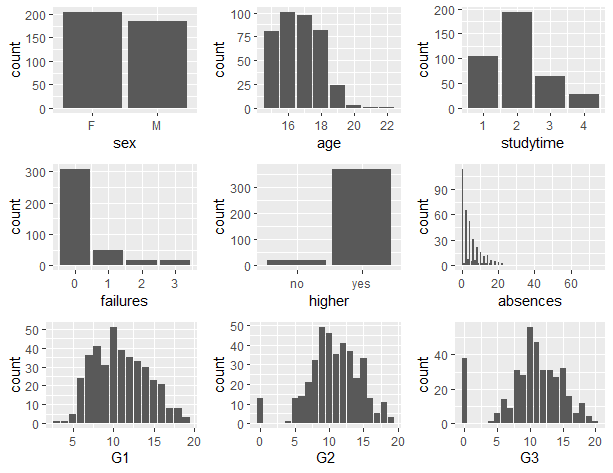
\includegraphics[width=0.8\textwidth]{hist.png}
\end{figure}

When it comes to box plot, we should only use it for categorical variables. Because of the nature of box plot it includes each category as an individual box so the categorical variables deliver just enough categories.
\begin{mdframed}[leftline=false,rightline=false,backgroundcolor=magenta!10,nobreak=true]
  \begin{minted}[linenos,breaklines,breaksymbolleft=,obeytabs=true,tabsize=2]{R}
# Box plot of G3 for sex, age, studytime, failures, higher
grid.arrange(
  ggplot(grade_csv, aes(x=as.character(sex), y=G3 )) + geom_boxplot() + scale_x_discrete(name="Sex"),
  ggplot(grade_csv, aes(x=as.character(age), y=G3)) + geom_boxplot() + scale_x_discrete(name="Age"),
  ggplot(grade_csv, aes(x=as.character(studytime), y=G3)) + geom_boxplot() + scale_x_discrete(name="Study time"),
  ggplot(grade_csv, aes(x=as.character(failures), y=G3)) + geom_boxplot() + scale_x_discrete(name="Failures"),
  ggplot(grade_csv, aes(x=as.character(higher), y=G3)) + geom_boxplot() + scale_x_discrete(name="Higher"),
  ncol = 2
)
  \end{minted}
\end{mdframed}

The corresponding output:

\begin{figure}[H]
  \centering
  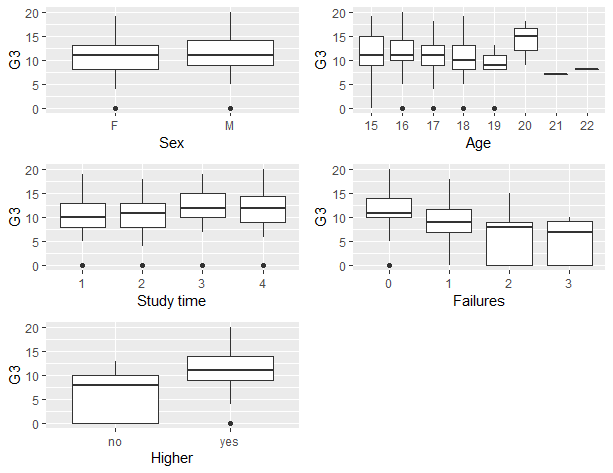
\includegraphics[width=0.8\textwidth]{boxplot.png}
\end{figure}

For pairing we will pair \(G3\) with \(age\), \(absences\), \(G1\) and \(G2\):
\begin{mdframed}[leftline=false,rightline=false,backgroundcolor=magenta!10,nobreak=true]
  \begin{minted}[linenos,breaklines,breaksymbolleft=,obeytabs=true,tabsize=2]{R}
pairs(G3 ~ G2, data = grade_csv)
pairs(G3 ~ G1, data = grade_csv)
pairs(G3 ~ age, data = grade_csv)
pairs(G3 ~ absences, data = grade_csv)
  \end{minted}
\end{mdframed}

Executing each line, there will be an individual plot shown on the screen and only one at a time. Here the results shown from different time are combined into a frame to ease the visualization step:

\begin{figure}[H]
  \centering
  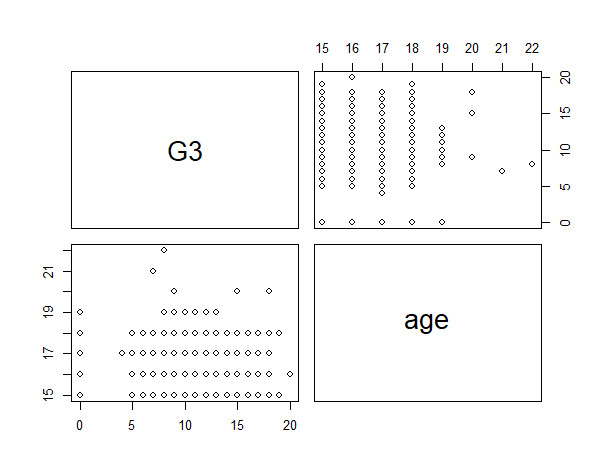
\includegraphics[width=0.4\textwidth]{pairs_age.png}
  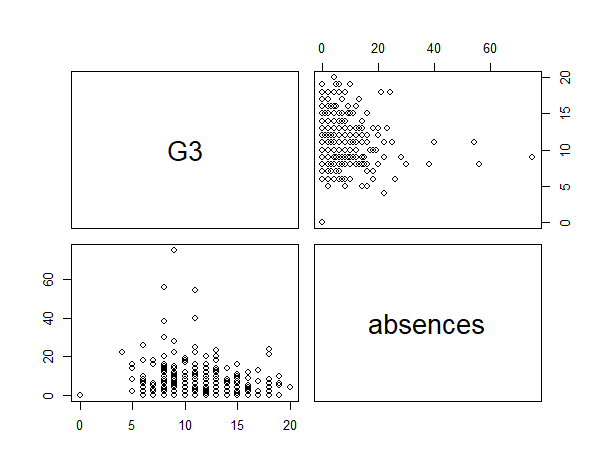
\includegraphics[width=0.4\textwidth]{pairs_ab.png}
  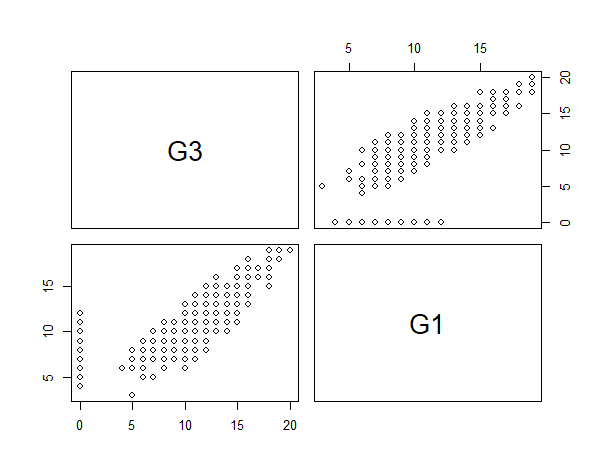
\includegraphics[width=0.4\textwidth]{pairs_g1.png}
  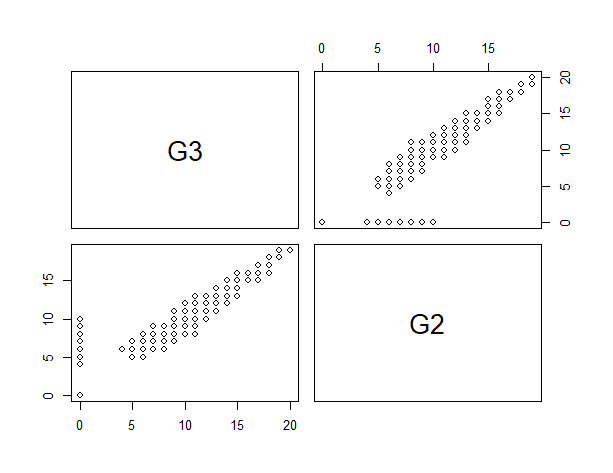
\includegraphics[width=0.4\textwidth]{pairs_g2.png}
\end{figure}

%%%%%%%%%%%%%%%%%%%%%%%%%%%%%%%%%

\subsubsection{Building linear regression models}
\begin{itemize}
  \item Consider a linear regression model that includes \(G3\) as a dependent variable, and all. The rest of the variables are all independent variables.
\end{itemize}

\begin{mdframed}[leftline=false,rightline=false,backgroundcolor=magenta!10,nobreak=true]
  \begin{minted}[linenos,breaklines,breaksymbolleft=,obeytabs=true,tabsize=2]{R}
M_all <- lm(G3 ~ sex + age + studytime + failures + higher + absences + G1 + G2, data = grade_csv)
summary(M_all)
  \end{minted}
\end{mdframed}

Obtain the result containing information, parameters for the regression program when we call the \mintinline{R}{summary()} function:
\begin{mdframed}[leftline=false,rightline=false,backgroundcolor=teal!10,nobreak=true]
  \begin{minted}[linenos,breaklines,breaksymbolleft=,obeytabs=true,tabsize=2]{text}
Call:
lm(formula = G3 ~ sex + age + studytime + failures + higher +
    absences + G1 + G2, data = grade_csv)

Residuals:
    Min      1Q  Median      3Q     Max
-9.1217 -0.4473  0.3160  0.9743  3.6379

Coefficients:
            Estimate Std. Error t value Pr(>|t|)
(Intercept)  0.61310    1.51569   0.405 0.686068
sexM         0.19679    0.20836   0.945 0.345511
age         -0.15235    0.08108  -1.879 0.061000 .
studytime   -0.13934    0.12477  -1.117 0.264810
failures    -0.19862    0.14784  -1.344 0.179909
higheryes    0.26384    0.47490   0.556 0.578836
absences     0.04208    0.01233   3.413 0.000711 ***
G1           0.16637    0.05696   2.921 0.003701 **
G2           0.96039    0.04994  19.231  < 2e-16 ***
---
Signif. codes:  0 ‘***’ 0.001 ‘**’ 0.01 ‘*’ 0.05 ‘.’ 0.1 ‘ ’ 1

Residual standard error: 1.912 on 381 degrees of freedom
Multiple R-squared:  0.8285,	Adjusted R-squared:  0.8249
F-statistic: 230.1 on 8 and 381 DF,  p-value: < 2.2e-16
  \end{minted}
\end{mdframed}

\begin{itemize}
  \item [-] At the bottom we see that \(F-statistics\) of our regression model has \(p-value < 0.05\) indicates that our model is significance compare to model only has intercept. And the value of \(R-squared\) that used to measured model quality approximate 0.8285 said that our model is quite good.

  \item[-] From the \(Estimate\) column we have Linear regression Equation:
        \begin{multline*}
          \textbf{G3} =  0.61310 + 0.19679\times \textbf{sex} + -0.15235\times \textbf{age} + \\
          -0.13934\times \textbf{studytime} + -0.19862\times \textbf{failures} + 0.26384\times \textbf{higher} + \\ 0.04208\times \textbf{higher} + 0.16637\times \textbf{G1} + 0.96039\times \textbf{G2}
        \end{multline*}
\end{itemize}

\begin{itemize}
  \item[-] Observing the p-value that is the value of \(\Pr(>|t|)\) in the Coefficients part. It's a probability that coefficient is insignificance in your model so smaller is better. Then we have t-test for:
\end{itemize}
\begin{itemize}
  \item[+] null-hypothesis \(H_{0}\): the coefficient is \textbf{insignificance} or this factor has no effect on the predictors
  \item[+] alternative-hypothesis \(H_{1}\): the coefficient is \textbf{significance} or this factor has effect on the predictors
        \begin{itemize}
          \item With \(\alpha = 0.05\)
                \begin{itemize}
                  \item \(P-value_{sex} = 0.345511 > 0.05\)
                  \item \(P-value_{age} = 0.061000 > 0.05\)
                  \item \(P-value_{studytime} = 0.264810 > 0.05\)
                  \item \(P-value_{failures} = 0.179909 > 0.05\)
                  \item \(P-value_{higher} = 0.578836 > 0.05\)
                \end{itemize}
        \end{itemize}

        We can see that the \(P-value_{age}\) is nearly close to 0.05 while others is very far from this value. Therefore we decide the factors that absolutely insignificance in the predictor are \(sex, studytime, failures, higher\). And after that we also keep \(age\) to examine that factor is have effect on the model or not.
\end{itemize}

\begin{itemize}
  \item We try to compare the model that contain all the independent variable with the model that we have just remove some insignificance factors from above to see whether 2 model that is perform the same effectiveness.
\end{itemize}
\begin{itemize}
  \item[-] We create model \(M1\) contain the dependent variables are \(age, absences, G1, G2\) and do ANOVA test to recommend the better linear regression model:
\end{itemize}
\begin{mdframed}[leftline=false,rightline=false,backgroundcolor=magenta!10,nobreak=true]
  \begin{minted}[linenos,breaklines,breaksymbolleft=,obeytabs=true,tabsize=2]{R}
####### -------> model just contain age, absences, G1, G2
M1 <- lm(G3 ~ age + absences + G1 + G2, data = grade_csv)
# anova between M_all and M1
anova(M_all, M1)
  \end{minted}
\end{mdframed}

\begin{itemize}
  \item [-] The result show that:
\end{itemize}
\begin{mdframed}[leftline=false,rightline=false,backgroundcolor=teal!10,nobreak=true]
  \begin{minted}[linenos,breaklines,breaksymbolleft=,obeytabs=true,tabsize=2]{text}
Analysis of Variance Table

Model 1: G3 ~ sex + age + studytime + failures + higher + absences + G1 + G2
Model 2: G3 ~ age + absences + G1 + G2
Res.Df    RSS Df Sum of Sq      F Pr(>F)
1    381 1392.4
2    385 1409.8 -4   -17.347 1.1866 0.3162
---
Signif. codes:  0 ‘***’ 0.001 ‘**’ 0.01 ‘*’ 0.05 ‘.’ 0.1 ‘ ’ 1
  \end{minted}
\end{mdframed}

\begin{itemize}
  \item[-] With the null-hypothesis \(H_0\): These two models M1 and M\_all perform the same effectiveness.
  With \(alpha = 5\% \) and observing from the ANOVA table we see that \(p-value = 0.3162 > 0.05\) then we \textbf{fail to reject null-hypothesis}. From that we can conclude that 2 model are perform the same effectiveness. Therefore, we \textbf{choose model M1 to continue} because it more simpler than M\_all to reduce cost of computation.
\end{itemize}

\begin{itemize}
  \item Then we examine the variable \(age\) that have effect on your model or not. We continue comparing model M1 with the model have been removed the factor age called M2.
\end{itemize}

\begin{mdframed}[leftline=false,rightline=false,backgroundcolor=magenta!10,nobreak=true]
  \begin{minted}[linenos,breaklines,breaksymbolleft=,obeytabs=true,tabsize=2]{R}
####### ---------> from model M1 we remove factor age
M2 <- lm(G3 ~absences + G1 + G2, data = grade_csv)
# anova between M1 and M2
anova(M1, M2)
  \end{minted}
\end{mdframed}

\begin{itemize}
  \item [-] The result show that:
\end{itemize}
\begin{mdframed}[leftline=false,rightline=false,backgroundcolor=teal!10,nobreak=true]
  \begin{minted}[linenos,breaklines,breaksymbolleft=,obeytabs=true,tabsize=2]{text}
Analysis of Variance Table

Model 1: G3 ~ age + absences + G1 + G2
Model 2: G3 ~ absences + G1 + G2
Res.Df    RSS Df Sum of Sq      F  Pr(>F)
1    385 1409.8
2    386 1430.7 -1    -20.95 5.7213 0.01724 *
---
Signif. codes:  0 ‘***’ 0.001 ‘**’ 0.01 ‘*’ 0.05 ‘.’ 0.1 ‘ ’ 1
  \end{minted}
\end{mdframed}
\begin{itemize}
  \item[-] With the null-hypothesis \(H_0\): These two models M1 and M2 perform the same effectiveness instead of M2 lacking the factor age. With \(alpha = 5\%\) and observing from the ANOVA table we see that \(p-value = 0.01724 < 0.05\) then we \textbf{reject null-hypothesis}. We can conclude that 2 model are perform the different effectiveness or significance. Which is also said that \textbf{factor age might affect the final grade G3}. Therefore, we are decide to \textbf{choose model M1 to be the most suitable model}.
  \item[-] We can see that if we decided to remove factor age from the beginning, we can nearly drop out some important factor from our datasets that might be affected to your model a lot.
\end{itemize}

\begin{itemize}
  \item Check if linear regression model M1 is appropriate for the data:
\end{itemize}

\begin{itemize}
  \item[-] We plot residual plot of model M1:
\end{itemize}

\begin{mdframed}[leftline=false,rightline=false,backgroundcolor=magenta!10,nobreak=true]
  \begin{minted}[linenos,breaklines,breaksymbolleft=,obeytabs=true,tabsize=2]{R}
## plot the residual plot
plot(M1)
  \end{minted}
\end{mdframed}
\begin{itemize}
  \item[-] We have plot figure:
\end{itemize}

\begin{figure}[H]
  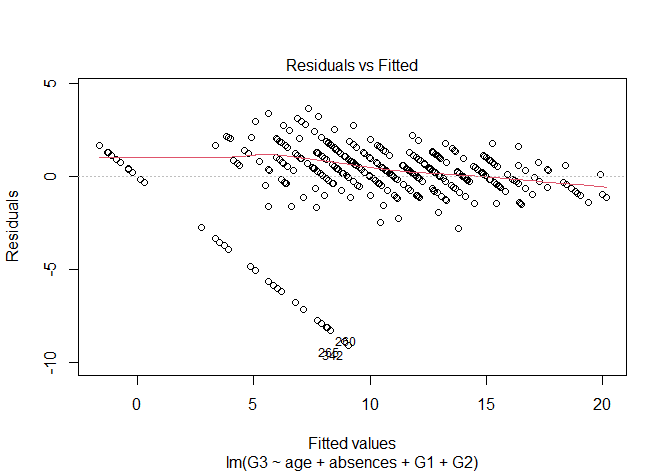
\includegraphics[scale = 0.7]{residual_plot.png}
\end{figure}


\begin{itemize}
  \item[-] Model's prediction is quite good, the linear regression (red line) is neighboring Residual = 0, the observed value concentrate around the read line and the residual plot do not have specific pattern. This is indicated that the model M1 we choose is sure-enough appropriate.
\end{itemize}


\begin{itemize}
  \item Inferring the effects of variable on the final grade G3 of model M1
  \item[-] Check the summary of model M1:

        \begin{mdframed}[leftline=false,rightline=false,backgroundcolor=magenta!10,nobreak=true]
          \begin{minted}[linenos,breaklines,breaksymbolleft=,obeytabs=true,tabsize=2]{R}
 summary(M1)
  \end{minted}
        \end{mdframed}
\end{itemize}

\begin{mdframed}[leftline=false,rightline=false,backgroundcolor=teal!10,nobreak=true]
  \begin{minted}[linenos,breaklines,breaksymbolleft=,obeytabs=true,tabsize=2]{text}
Call:
lm(formula = G3 ~ age + absences + G1 + G2, data = grade_csv)

Residuals:
    Min      1Q  Median      3Q     Max
-9.0758 -0.4018  0.3342  1.0086  3.6469

Coefficients:
            Estimate Std. Error t value Pr(>|t|)
(Intercept)  1.02355    1.35932   0.753 0.451920
age         -0.18710    0.07822  -2.392 0.017239 *
absences     0.04173    0.01227   3.401 0.000742 ***
G1           0.17481    0.05617   3.112 0.001994 **
G2           0.96720    0.04983  19.409  < 2e-16 ***
---
Signif. codes:  0 ‘***’ 0.001 ‘**’ 0.01 ‘*’ 0.05 ‘.’ 0.1 ‘ ’ 1

Residual standard error: 1.914 on 385 degrees of freedom
Multiple R-squared:  0.8264,	Adjusted R-squared:  0.8246
F-statistic: 458.2 on 4 and 385 DF,  p-value: < 2.2e-16
  \end{minted}
\end{mdframed}

\begin{itemize}
  \item[-] For assessing the effects of factor on the final grade G3, we must consider about each p-value for each factor. We see that the p-value corresponding to factor G2 and absences (***) < 0.001, this says that the second period grade and number of school absences have extremely impact on the final grade G3. We see that the p-value of first period grade G1(**) < 0.01 and student's age(*) < 0.05 also have impact on final grade G3 but it is lesser than G2 and absences. The rest of factor are sex, studytime, failures, higher have no significance impact on G3 so we do not consider in inside model.

  \item[-] The other side, the coefficient of independent variable might affect predictor. Assuming when you increase 1 unit of any independent variables and the rest of independent variable is constant then the bigger of coefficient the bigger expected value of predictor.
\end{itemize}

\newpage
%%%%%%%%%%%%%%%%%%%%%%%%%%%%%%%%%

\subsubsection{Predicting results}
\begin{itemize}
  \item[-] In general, the score is must larger than the mean overall score indicate that the student is pass, otherwise is fail. In this dataset, we are assuming is 10 is the value for classify student Fail or Pass.
\end{itemize}

\begin{itemize}
  \item[-] We create function to check student fail or pass with input is the grade
\end{itemize}

\begin{mdframed}[leftline=false,rightline=false,backgroundcolor=magenta!10,nobreak=true]
  \begin{minted}[linenos,breaklines,breaksymbolleft=,obeytabs=true,tabsize=2]{R}
## we want to create a function to check fail or pass of student
failpass <- function(x) {
  if (x >= 10)
    return("Pass") # x >= 10 Pass
  else
    return("Fail") # x < 10 Fail
}
  \end{minted}
\end{mdframed}

\begin{itemize}
  \item[-] With the most appropriate model that we have choose is M1. We create a new table and use the command \mintinline{R}{predict()} to get the predicted value of final grade G3 with the input from model M1 and evaluate it with our fuction:
\end{itemize}

\begin{mdframed}[leftline=false,rightline=false,backgroundcolor=magenta!10,nobreak=true]
  \begin{minted}[linenos,breaklines,breaksymbolleft=,obeytabs=true,tabsize=2]{R}
## create a new table and add predict column to a new table
new_grade <- grade_csv
predict_G3 <- predict(M1)
new_grade <- cbind(new_grade, predict_G3)
## check fail or pass of prediction in new table
predict_evaluate <- c(apply(new_grade["predict_G3"], MARGIN = 1, FUN = failpass))
new_grade <- cbind(new_grade, predict_evaluate)
  \end{minted}
\end{mdframed}

Let's see what new\_grade contain after binding predict\_evaluate column into it:

\begin{center}
  \makebox[\textwidth]{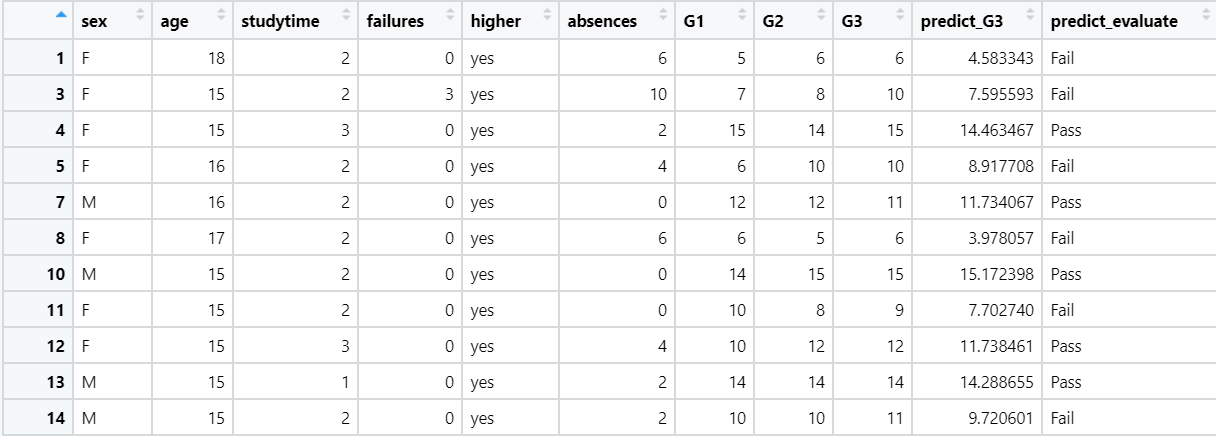
\includegraphics[width=\textwidth]{evaluate_predict.PNG}}
\end{center}


\begin{itemize}
  \item[-] Evaluate the final grade G3 of observed value:
\end{itemize}

\begin{mdframed}[leftline=false,rightline=false,backgroundcolor=magenta!10,nobreak=true]
  \begin{minted}[linenos,breaklines,breaksymbolleft=,obeytabs=true,tabsize=2]{R}
## Check G3 column fail or pass and add it to column evaluate
evaluate <- c(apply(grade_csv["G3"], MARGIN = 1, FUN = failpass))
grade_csv <- cbind(grade_csv, evaluate)
  \end{minted}
\end{mdframed}

Let's see what grade\_csv contain after binding evaluate column into it:

\begin{center}
  \makebox[\textwidth]{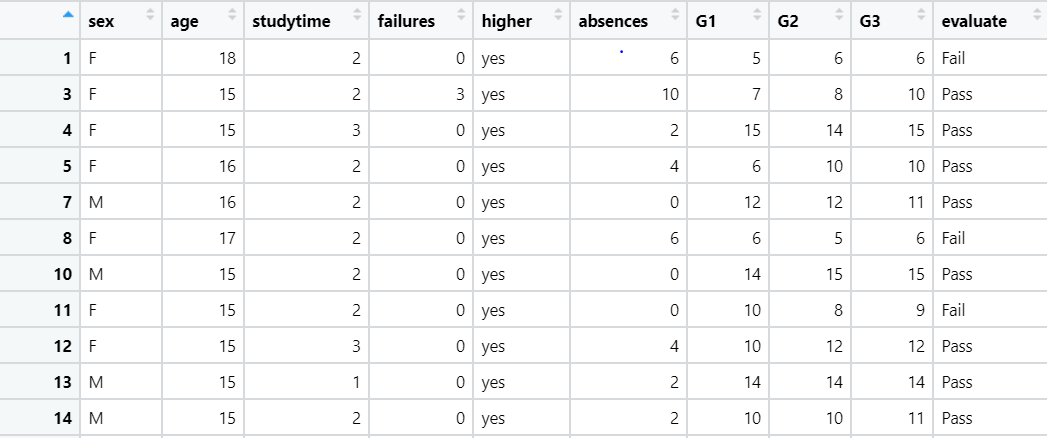
\includegraphics[width=\textwidth]{evaluate_observed.PNG}}
\end{center}

\begin{itemize}
  \item[-] We are assessing the precision through out the prediction by creating a table to compare the result between G3 and predict\_G3. By using the above function to check whether student can fail or pass, we can compare the proportion of Fail and Pass between G3 and predict\_G3
\end{itemize}

\begin{mdframed}[leftline=false,rightline=false,backgroundcolor=magenta!10,nobreak=true]
  \begin{minted}[linenos,breaklines,breaksymbolleft=,obeytabs=true,tabsize=2]{R}
## create a data frame to compare between G3(real data) and predicted value
evaluate1 = prop.table(table(grade_csv$evaluate == "Pass"))
evaluate2 = prop.table(table(new_grade$predict_evaluate == "Pass"))
Output = data.frame(cbind(evaluate1, evaluate2))
colnames(Output) = c("Real", "Predicted")
rownames(Output) = c("Fail", "Pass")
Output
  \end{minted}
\end{mdframed}

The proportion of Fail and Pass between the observed and predicted value:

\begin{center}
  {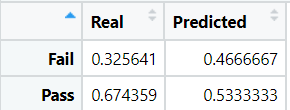
\includegraphics{proportion.PNG}}
\end{center}

\begin{itemize}
  \item[-] \textbf{Conclusion:} Depending on the result we have obtained between the observed and predicted value about the proportion of student Fail or Pass, we see that appear a insignificant different between the observed and predicted value. The reason might be caused by the outliers of the datasets so they effect the final prediction. However in general, these value still can be accepted. We do not remove outliers out of datasets because when I do this, the model might be leaved out some special case that importance for others research.
\end{itemize}

\newpage
%%%%%%%%%%%%%%%%%%%%%%%%%%%%%%%%%

\end{document}
